\chapter{Variabilité du bois}\label{variabilite}

\begin{abstract}
Dans ce chapitre, nous décrivons la variabilité des propriétés du bois aux échelles suivantes: 1) dans un même cerne annuel, de la moëlle vers l'écorce et 3) selon la position au long de la tige. Nous nous attardons tant aux caractéristiques anatomiques (longueur et diamètre des cellules de bois) qu'à la composition chimique et aux propriétés physico-mécaniques. Un résumé de toutes le notions est inclus à la toute fin du chapitre.
\end{abstract}

\minitoc

\section{Introduction}

On fait souvent l'erreur de croire que le bois produit par des arbres de la même espèce est identique au niveau de sa structure et de ses caractéristiques physiques. En fait, le bois produit par des arbres de la même espèce et même le bois de deux pièces provenant du même arbre peut être très différent à plusieurs points de vue : masse volumique, accroissement annuel, dimension des cellules, épaisseur des parois cellulaires, constituants chimiques, angle des microfibrilles, nombre et taille des nœuds, rectitude du fil, résistance mécanique, perméabilité.\\

La \og qualité \fg du bois pour une utilisation donnée est déterminée par la variabilité d'une ou plusieurs de ces caractéristiques et de son impact sur cette utilisation. Les causes de ces variations peuvent se résumer comme suit :

\begin{enumerate}
\item Les changements du cambium vasculaire avec l'âge;
\item Le bagage génétique;
\item L'environnement.
\end{enumerate}

\section{Variabilité du bois à l'intérieur d'un arbre}

La variabilité du bois à l'intérieur des arbres et entre les arbres de la même espèce est encore peu connue pour les espèces commerciales résineuses et feuillues du Québec. Toutefois, des efforts de recherche sont présentement consentis dans ce domaine. La variabilité du bois dans un arbre dépend principalement de deux facteurs :

\begin{enumerate}
\item Le vieillissement du cambium;
\item Les variations de l'activité du cambium.
\end{enumerate}

\subsection{Variabilité des dimensions des cellules dans la section transversale des tiges}

Des variations importantes et claires sont observables chez les cellules où une élongation post-cambiale est présente, c'est-à-dire chez les trachéides, les fibres et les éléments de vaisseaux. Des variations moins accentuées sont observables dans la section des cellules, l'épaisseur des parois cellulaires et l'angle des microfibrilles dans les parois cellulaires.

\subsubsection{Longueur des trachéides des résineux et des fibres des feuillus dans le cerne annuel}

Les trachéides des résineux et les fibres des feuillus ont une longueur minimale dans le bois initial et maximale dans le bois final. La longueur est généralement en décroissance à la fin du cerne annuel (Figures ~\ref{fig:long_cerne} à \ref{fig:long_mfa_cerne}).

\begin{figure}[h]
	\centering
	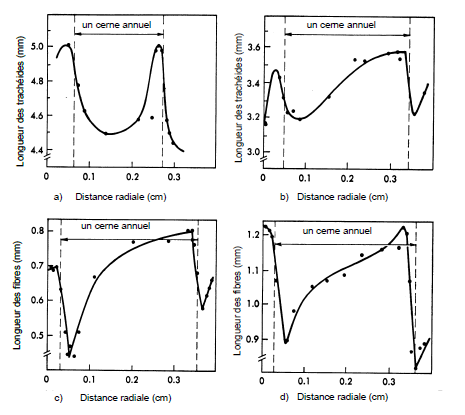
\includegraphics[scale=0.8]{img/ch7_long_cerne}
	\caption{Variation de la longueur des cellules du bois initial au bois final à l'intérieur d'un cerne annuel. a) longueur des trachéides chez Pseudotsuga menziesii (résineux à transition abrupte), b) longueur des trachéides chez Pinus radiata (résineux à transition graduelle), c) longueur des fibres chez Catalpa bignonioides (feuillu à zone poreuse), d) longueur des fibres chez Populus tremuloides (feuillu à pores diffus) (adapté de \cite{panshin1980textbook})}
	\label{fig:long_cerne}
\end{figure}

\subsubsection{Longueur des éléments de vaisseaux dans le cerne annuel}

Chez les bois à zone poreuse, les éléments de vaisseaux sont courts dans le bois initial et longs dans le bois final (Figure~\ref{fig:long_fibres_cerne}). La longueur des éléments de vaisseaux est donc inversement proportionnelle au diamètre de ces derniers. Chez les bois à pores diffus, on observe une légère augmentation de la longueur des éléments de vaisseaux du bois initial au bois final (Figure~\ref{fig:long_diffus_cerne}).


\begin{figure}[h]
	\centering
	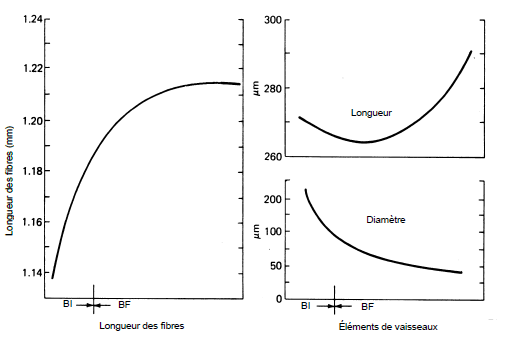
\includegraphics[scale=0.7]{img/ch7_long_fibres_cerne}
	\caption{Variation de la dimension des cellules à l'intérieur d'un cerne annuel de bois mature d'un bois feuillu à zone poreuse \textit{Fraxinus pennsylvanica} (adapté de \cite{panshin1980textbook})}
	\label{fig:long_fibres_cerne}
\end{figure}

\begin{figure}[h]
	\centering
	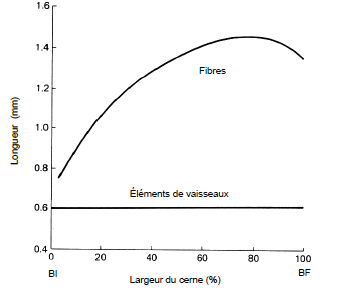
\includegraphics[scale=0.8]{img/ch7_long_diffus_cerne}
	\caption{Longueur des fibres et des éléments de vaisseaux à l'intérieur d’un cerne annuel de bois mature d'un bois feuillu à pores diffus, \textit{Fagus sylvatica} (adapté de \cite{panshin1980textbook})}
	\label{fig:long_diffus_cerne}
\end{figure}

\begin{figure}[h]
	\centering
	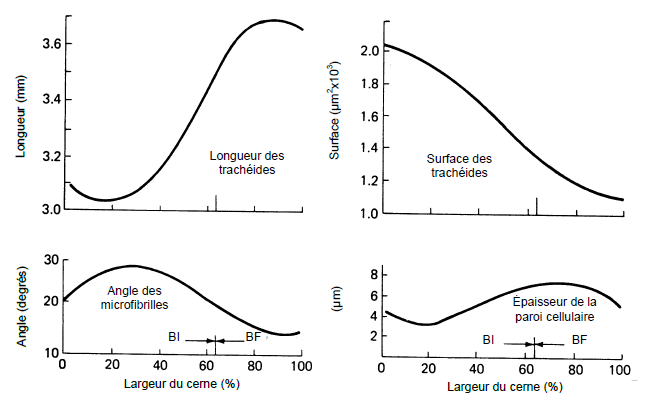
\includegraphics[scale=0.7]{img/ch7_long_mfa_cerne}
	\caption{Variation des dimensions des cellules et des angles des microfibrilles dans le cerne annuel d'un bois résineux à transition abrupte (adapté de \cite{panshin1980textbook})}
	\label{fig:long_mfa_cerne}
\end{figure} 


\subsubsection{Section des cellules dans le cerne annuel}

La section (surface) des cellules diminue du bois initial au bois final. Chez les résineux, en raison de l'alignement radial des trachéides, c'est la dimension des trachéides en direction radiale qui tend à varier (Figure~\ref{fig:resume_resineux}). Chez les feuillus à zone poreuse et semi-poreuse, on observe une diminution en diamètre des vaisseaux sans orientation particulière (Figure~\ref{fig:long_fibres_cerne}).

\subsubsection{Angle des microfibrilles des parois cellulaires dans le cerne annuel}

L'angle des microfibrilles des parois cellulaires est inversement proportionnel à la longueur des cellules. Il est donc maximal dans le bois initial et minimal dans le bois final (Figure~\ref{fig:long_mfa_cerne}).

\subsubsection{Variabilité de la structure du bois entre les cernes annuels}

On observe des variations nettes des caractéristiques du bois de la moelle vers l'écorce. Les causes de ces variations sont principalement :

\begin{enumerate}
\item Les changements des initiales du cambium avec le vieillissement de ce dernier;
\item le développement post-cambial des cellules.
\end{enumerate}

Cela engendre des variations dans :	

\begin{itemize}
\item dimensions des cellules;
\item structure de la paroi cellulaire incluant l'angle des microfibrilles;
\item proportion du volume occupé par différents types de cellules;
\item composition chimique des parois cellulaires.
\end{itemize}

Qui ont pour conséquences des changements dans les propriétés du bois :

\begin{itemize}
\item masse volumique;
\item résistance mécanique;
\item retrait et gonflement;
\item autres\ldots
\end{itemize}

Ces variations dans la section transversale en direction radiale et selon l'axe de la tige sont assez constantes d'une tige à l'autre, autant chez les résineux que chez les feuillus.

\subsubsection{Variation de la longueur des cellules dans le plan transversal des tiges}

On observe en général une élongation rapide des fibres et des trachéides dans les premières années de croissance (Figure~\ref{fig:long_moelle}). Il s'agit alors du bois juvénile. Suite à la période de production du bois juvénile, le cambium mature produit du bois selon les trois caractéristiques suivantes :

\begin{enumerate}
\item Stabilisation de la longueur des cellules;
\item Augmentation continue de la longueur des cellules;
\item Courbes paraboliques montrant une diminution de la longueur des cellules
\end{enumerate}

\begin{figure}[h]
	\centering
	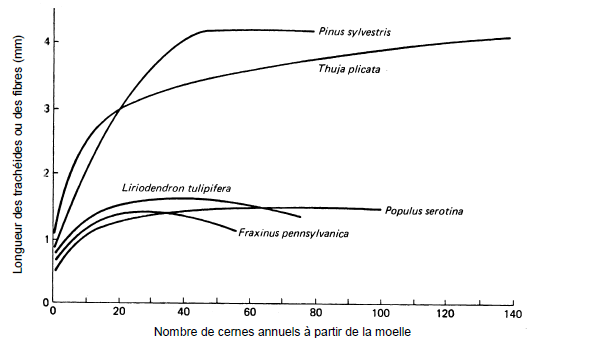
\includegraphics[scale=0.7]{img/ch7_long_moelle}
	\caption{Courbes typiques illustrant la longueur des cellules de la moelle vers l'écorce (adapté de \cite{panshin1980textbook})}
	\label{fig:long_moelle}
\end{figure}


D'autre part, notons les points suivants :

\begin{itemize}
\item La période juvénile se termine habituellement après 10 à 20 ans dans le climat de l'Est du Canada. 
\item En général, la longueur des fibres et des trachéides diminue chez les arbres surannés. 
\item Les fibres et les trachéides sont toujours plus courtes dans le bois initial que dans le bois final.
\item La longueur des fibres et des trachéides varie en fonction de la hauteur dans l'arbre (Figure~\ref{fig:long_haut_resume}).
\item Les éléments de vaisseaux augmentent en longueur de la moelle vers l'écorce mais moins que les fibres puisque les éléments de vaisseaux croissent davantage en directions radiale et tangentielle dans la zone cambiale (Figure~\ref{fig:long_moelle_feuillus}).
\end{itemize}

La variation en longueur des éléments de vaisseaux, des fibres et des trachéides est due : 1) à la variation en longueur des initiales du cambium et 2) au développement post-cambial des cellules.

\begin{figure}[h]
	\centering
	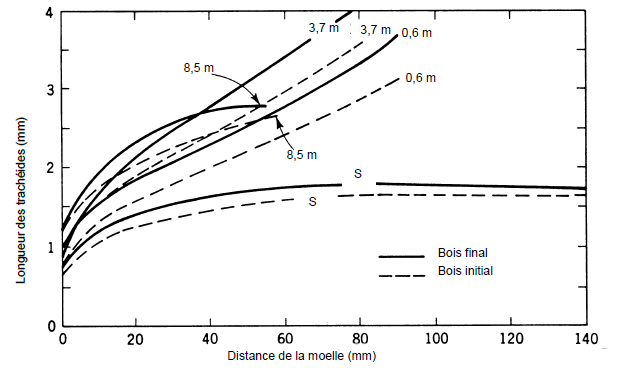
\includegraphics[scale=0.7]{img/ch7_long_haut_resume}
	\caption{Variation de la longueur des trachéides selon la hauteur dans la tige pour le bois initial et le bois final dans une tige de pin rouge (\textit{Pinus resinosa}) de 35 ans. Les plus courtes trachéides se retrouvent au niveau du sol (S). La longueur des trachéides augmente rapidement jusqu'à une hauteur de 0,6 m. L'augmentation en longueur continue jusqu'à une longueur maximale sous la cime vivante (3,7 m) et décroît alors jusqu'au sommet de la cime vivante. Les courbes du bois initial montrent des trachéides plus courtes dans tous les cas (adapté de \cite{panshin1980textbook})}
	\label{fig:long_haut_resume}
\end{figure}

\begin{figure}[h]
	\centering
	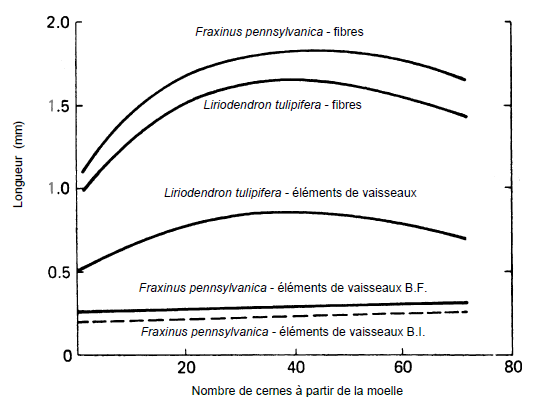
\includegraphics[scale=0.7]{img/ch7_long_moelle_feuillus}
	\caption{Variation de la longueur des fibres et des éléments de vaisseaux de la moelle vers l'écorce (adapté de \cite{panshin1980textbook})}
	\label{fig:long_moelle_feuillus}
\end{figure}

\subsubsection{Variation du diamètre des cellules de la moelle vers l'écorce}

\begin{itemize}
	\item Chez les résineux, la section des trachéides augmente de la moelle vers l'écorce (Figure~\ref{fig:resume_resineux});
	\item Le volume des trachéides augmente de la moelle vers l'écorce puisque la section et la longueur augmentent;
	\item Chez les feuillus, les éléments de vaisseaux s'accroissent en diamètre de la moelle vers l'écorce, autant chez les bois à pores diffus qu'à zone poreuse; 
	\item Chez les feuillus, les fibres s'accroissent en diamètre modérément ou ce diamètre demeure constant de la moelle vers l'écorce, autant chez les bois à pores diffus qu'à zone poreuse.
\end{itemize}

\subsubsection{Variation de l'épaisseur des parois cellulaires de la moelle vers l'écorce}

Chez les résineux, l'épaisseur des parois du bois final augmente progressivement au moins jusqu'à 30 ans (environ 40\%), l'épaisseur des parois du bois initial augmente aussi mais de façon moins prononcée (environ 20\%) et on a une augmentation en épaisseur selon la direction radiale surtout.\\

Chez les feuillus on a une augmentation de l'épaisseur des parois de la moelle vers l'écorce.

\begin{figure}[h]
	\centering
	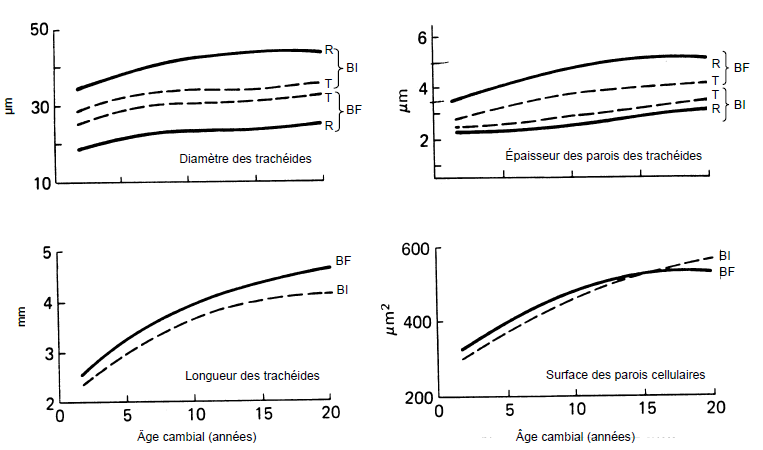
\includegraphics[scale=0.7]{img/ch7_resume_resineux}
	\caption{Variation des dimensions des trachéides de la moelle vers l'écorce chez de jeunes arbres de \textit{Pinus radiata} \cite{panshin1980textbook})}
	\label{fig:resume_resineux}
\end{figure}


\subsubsection{Variation de l'angle des microfibrilles de la moelle vers l'écorce}

L'angle des microfibrilles dans les parois cellulaires des trachéides et des fibres est inversement proportionnel à la longueur des cellules (Figure~\ref{fig:long_mfa_moelle}). Donc, l'angle des microfibrilles change de la moelle vers l'écorce avec les changements de longueur des trachéides ou des fibres.

\begin{figure}[h]
	\centering
	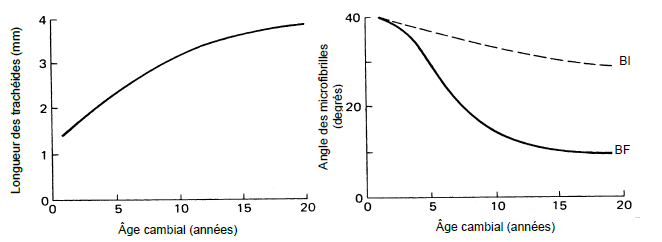
\includegraphics[scale=0.8]{img/ch7_long_mfa_moelle}
	\caption{Variation de la longueur des trachéides et de l'angle des microfibrilles de la moelle vers l'écorce dans les parois cellulaires de \textit{Cryptomeria japonica} (Cèdre du Japon ou Sugi) \cite{panshin1980textbook})}
	\label{fig:long_mfa_moelle}
\end{figure}

\subsection{Variabilité des dimensions des cellules selon la hauteur des tiges}

\subsubsection{Variation de la longueur des cellules selon la hauteur}

De façon générale, on peut dire que la longueur maximale des trachéides ou des fibres est localisée dans la partie extérieure du tronc, à environ 1/3 à 1/2 de la hauteur de l'arbre. Il y a des exceptions à cette règle. Par exemple, chez le sapin Douglas la longueur des trachéides augmente du bas vers le haut de l'arbre.

\subsubsection{Variation du diamètre des cellules}

En général, le diamètre des trachéides des résineux augmente de la souche jusqu'à environ le tiers à la demie de la hauteur de l'arbre et il diminue par la suite jusqu'au sommet de la cime vivante.\\

En général, le diamètre des fibres des feuillus diminue de la base jusqu'au sommet de la cime vivante.

\subsubsection{Variation de l'épaisseur des parois cellulaires}

L'épaisseur des parois cellulaires varie de la même façon que le diamètre des cellules, c'est-à-dire qu'en général, l'épaisseur des parois des trachéides des résineux augmente de la souche jusqu'à environ le tiers à la demie de la hauteur de l'arbre et elle diminue par la suite jusqu'au sommet de la cime vivante.\\

L'épaisseur des parois des fibres des feuillus diminue de la base jusqu'au sommet de la cime vivante.
%

%\begin{figure}[h]
%	\centering
	%	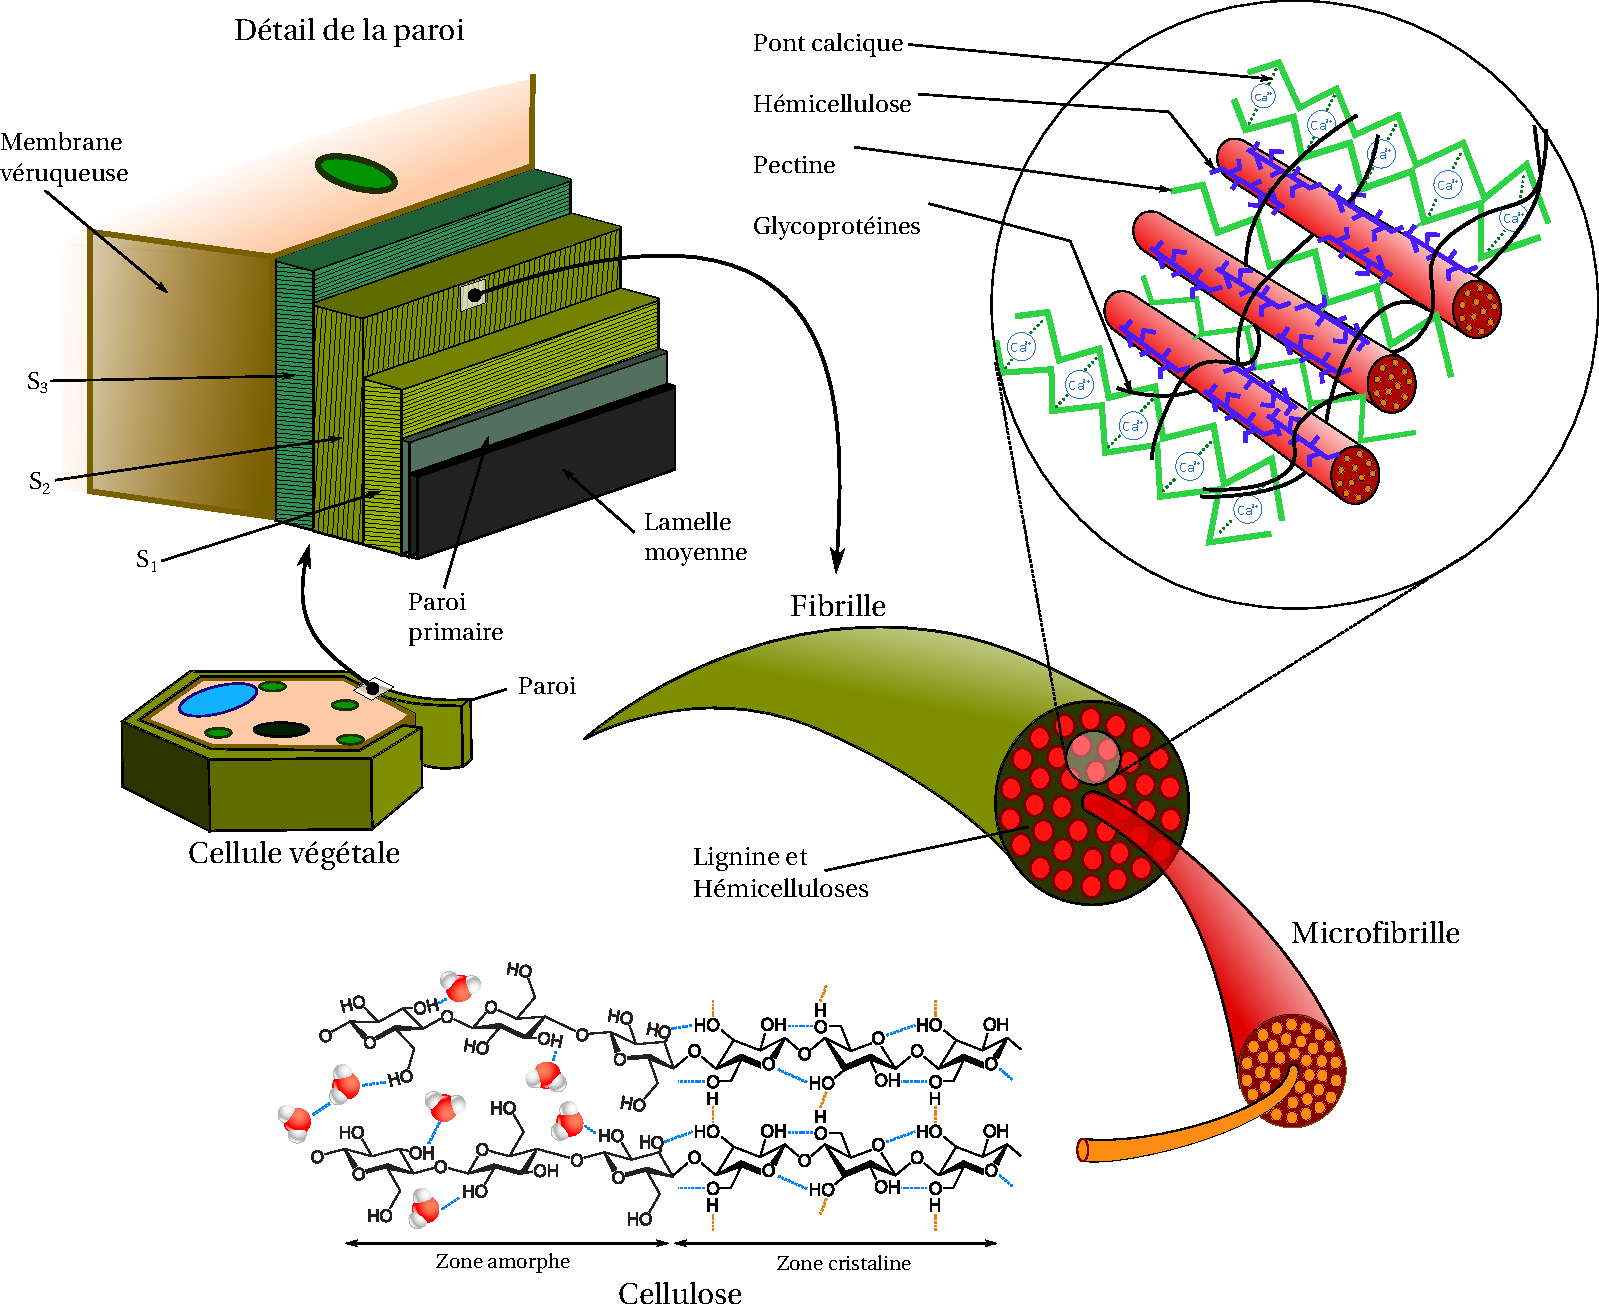
\includegraphics[scale=0.55]{img/ch6_cellule}
%	\caption{Variation de la longueur des fibres dans le plan longitudinal-radial d'une tige d'Eucalyptus regnans. Les deux côtés de la figure présentent les mêmes données de façon différente \cite{panshin1980textbook})}
%	%	\label{fig:grosschema}
%\end{figure}

\subsection{Dimensions des cellules dans les branches et les racines}

Les parties non commerciales des tiges (branches, racines, houppier) constituent environ 25\% de la masse anhydre des arbres. Il est donc pertinent de s'interroger sur les caractéristiques de ce bois.


\subsubsection{Variation des dimensions des cellules dans les branches}

Dans les résineux les trachéides sont significativement plus courtes dans les branches que dans la tige (50\% plus courtes) (Figure~\ref{fig:long_tige_branches}). Leur longueur atteint un maximum à environ un quart de la longueur de la branche et diminue par la suite.\\

Dans les feuillus la longueur des fibres des branches est d'environ 75\% de la longueur des fibres de la tige.

\subsubsection{Variations des dimensions des cellules dans les racines}

Dans les résineux, au collet, les trachéides sont courtes et il n'y a pas de variation radiale de longueur. La longueur des trachéides augmente du collet vers le bout des racines. Les trachéides des racines sont 50\% plus longues que celles de la tige en moyenne. Les trachéides des racines sont 30\% plus larges en direction tangentielle et les parois sont 15\% plus minces.

Dans les feuillus, les fibres des racines des feuillus sont environ 10\% plus courtes que celles des tiges.

\begin{figure}[h]
	\centering
	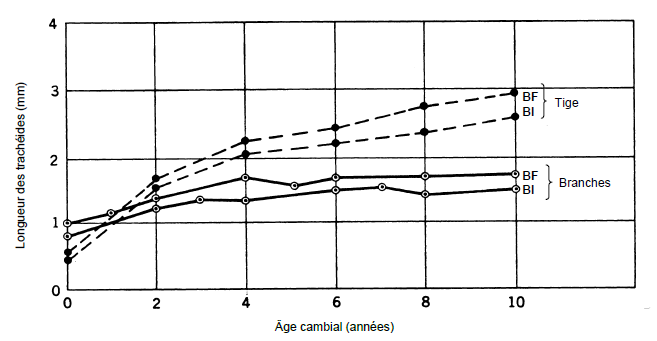
\includegraphics[scale=0.7]{img/ch7_long_tige_branches}
	\caption{Longueur des trachéides en fonction de l'âge cambial dans la tige et les branches de pin rouge (\textit{Pinus resinosa}) \cite{panshin1980textbook})}
	\label{fig:long_tige_branches}
\end{figure}

\section{Variation de la composition chimique des parois cellulaires}

\subsection{Polysaccharides}

\subsubsection{Teneur en cellulose}

Chez les résineux elle représente 40\% de la masse anhydre du bois initial et 50\% de la masse anhydre du bois final (Figure~\ref{fig:cellulose_cerne}). La cellulose du bois final possède un degré de polymérisation plus élevé et est plus cristalline que celle du bois initial. La teneur en cellulose des parois cellulaires augmente de la moelle vers l'écorce (45 à 65\% de la masse anhydre) (Figure~\ref{fig:cellulose_moelle}).

\subsubsection{Teneur en hémicelluloses}

Diminue de la moelle vers l'écorce (Figure~\ref{fig:cellulose_moelle}).

\subsection{Lignine}

Variations mineures en général. Elle varie de manière sinusoïdale dans le cerne annuel (Figure~\ref{fig:cellulose_cerne}) et tend à diminuer de la moelle vers l'écorce (Figure~\ref{fig:cellulose_moelle}).

\begin{figure}[h]
	\centering
	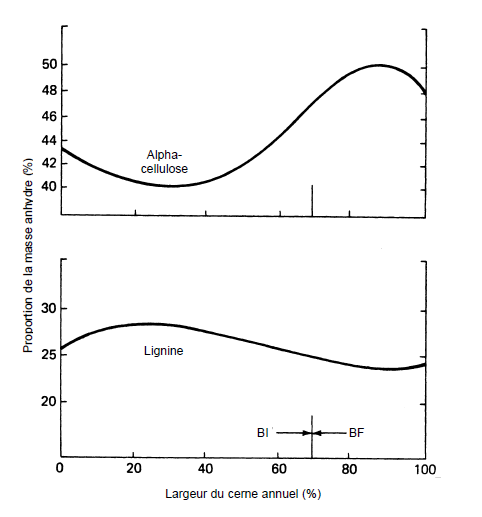
\includegraphics[scale=0.7]{img/ch7_cellulose_cerne}
	\caption{Variation de la teneur en cellulose et en lignine dans un cerne annuel de sapin Douglas (\textit{Pseudotsuga menziesii}) \cite{panshin1980textbook})}
	\label{fig:cellulose_cerne}
\end{figure}

\begin{figure}[h]
	\centering
	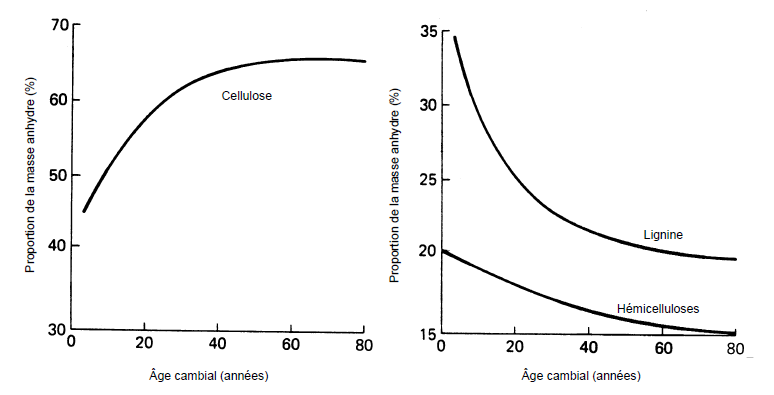
\includegraphics[scale=0.55]{img/ch7_cellulose_moelle}
	\caption{Distribution des composés chimiques de la paroi cellulaire de la moelle vers l'écorce chez les résineux \cite{panshin1980textbook})}
	\label{fig:cellulose_moelle}
\end{figure}


\section{Variation des propriétés physiques du bois}

\subsection{Variation de la masse volumique}

La masse volumique est définie comme la masse de matière par unité de volume. Elle est le plus important indicateur de qualité du bois et est principalement le résultat de variations de la structure cellulaire qui seront décrites ci-dessous.

\subsubsection{Variation de la masse volumique dans les cernes annuels}

Chez les résineux, la masse volumique est maximale dans le bois final et minimale dans le bois initial. La pente de la courbe $M_v$ en fonction de la position dans un cerne annuel dépend du type de transition bois initial / bois final. Le ratio $M_v$ bois final / $M_v$ bois initial = 2,5 à 5,0. Le bois initial est produit pendant la croissance des rameaux alors que la production d'auxines est maximale.  La transition bois initial / bois final correspond à l'arrêt de la croissance en longueur des rameaux.\\

L'augmentation de $M_v$ du bois final chez les résineux est principalement due à l'augmentation de l'épaisseur des parois cellulaires. Cette dernière résulte de la physiologie de l'arbre. Au début de la saison de croissance, les produits de la photosynthèse sont utilisés en priorité pour la croissance des rameaux et la production des aiguilles. Un minimum de substances nutritives est donc disponible au niveau du cambium.  En conséquence, les parois cellulaires demeurent minces jusqu'à ce que la croissance en longueur des rameaux cesse et que davantage de substances nutritives soient disponibles au niveau du cambium.

Chez les feuillus, la distribution des différents types de cellules (vaisseaux, fibres, parenchymes) détermine les variations de masse volumique dans le cerne annuel. De manière générale, la masse volumique est minimale dans le bois initial et maximale dans le bois final pour les feuillus à zone poreuse, à zone semi-poreuse et à pores diffus.
%
\subsubsection{Variation de la masse volumique de la moelle vers l'écorce}

Trois types :

\begin{description}
\item[Type I] Augmentation de $M_v$ de la moelle vers l'écorce;
\item[Type II] $M_v$ décroît à partir de la moelle mais s'accroît en s'approchant de l'écorce;
\item[Type III] $M_v$ décroît de la moelle vers l'écorce;
\end{description}


\subsubsection{Une espèce peut avoir différents types de comportement}

\textbf{Chez les résineux} les facteurs à considérer sont le diamètre des trachéides, l'épaisseur des parois et la proportion du cerne annuel occupée par le bois initial. Chez la plupart des espèces, la largeur de la bande de bois final varie moins que celle de bois initial (Figure~\ref{fig:larg_moelle}). On a donc des variations de $M_v$ (Figure~\ref{fig:densite_moelle}), car la proportion de bois final dans les cernes annuels change de la moelle vers l'écorce. L'épaisseur des parois augmente donc plus vite que le diamètre des trachéides.\\

\begin{figure}[h]
	\centering
	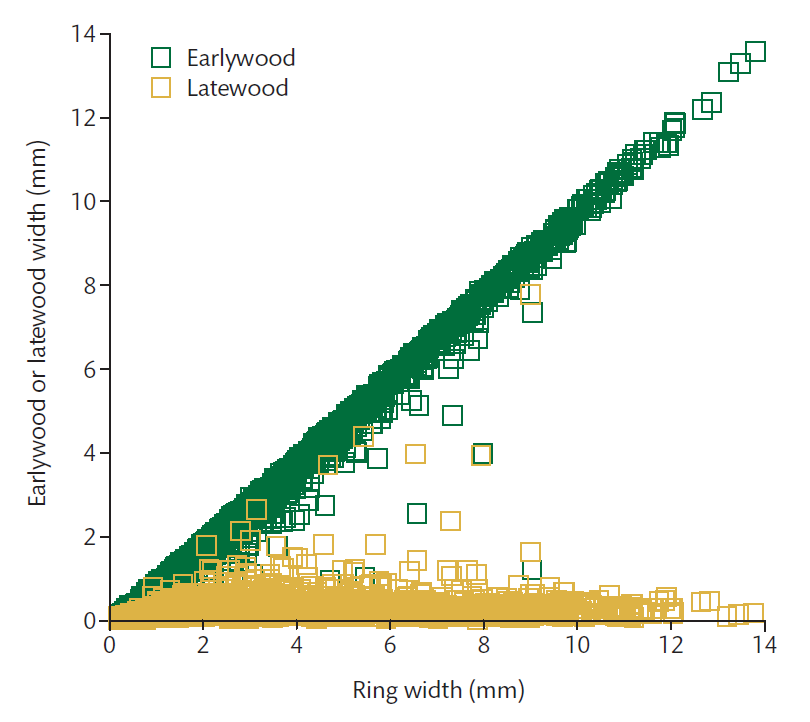
\includegraphics[scale=0.4]{img/ch7_larg_moelle}
	\caption{Largeur du bois initial et du bois final en fonction de la largeur totale du cerne chez l'épinette de Sitka \textit{Picea sitchensis} (\cite{moore2011wood})}
	\label{fig:larg_moelle}
\end{figure}

\begin{figure}[h]
	\centering
	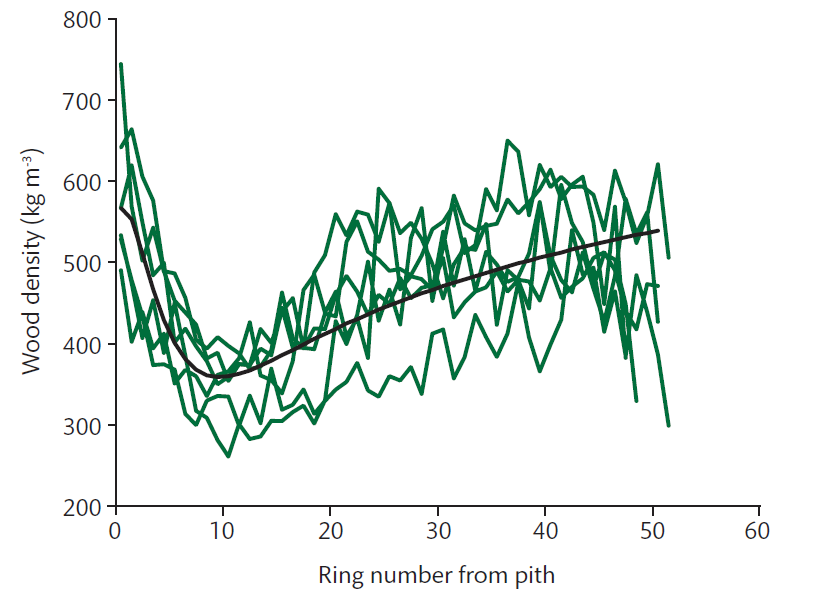
\includegraphics[scale=0.5]{img/ch7_densite_moelle}
	\caption{Parton typique de variation de la masse volumique de la moelle vers l'écorce cerne chez l'épinette de Sitka \textit{Picea sitchensis}. Le gain de densité près ce l'écorce s'explique par une diminution de la largeur des cernes. Ce patron de variation correspond au Type II (graphique reproduit de \cite{moore2011wood})}
	\label{fig:densite_moelle}
\end{figure}

\textbf{Chez les feuillus à zone poreuse}, la proportion de bois final varie car la largeur du bois initial est plus ou moins constante d'un cerne à l'autre. Donc, si la largeur du cerne augmente, $M_v$ augmente et inversement (Figure~\ref{fig:densite_moelle_feuillus}).\\

\textbf{Chez les feuillus à pores diffus}, la proportion vaisseaux/fibres est le facteur déterminant (Figure~\ref{fig:densite_moelle_feuillus}). Le diamètre des vaisseaux augmente et le nombre de vaisseaux par unité de surface diminue de la moelle vers l'écorce. $M_v$ augmente si la proportion de fibres augmente. $M_v$ augmente si l'épaisseur des parois des fibres augmente. $M_v$ diminue si le diamètre des vaisseaux augmente avec une diminution de l'épaisseur des parois des fibres.

\begin{figure}[h]
	\centering
	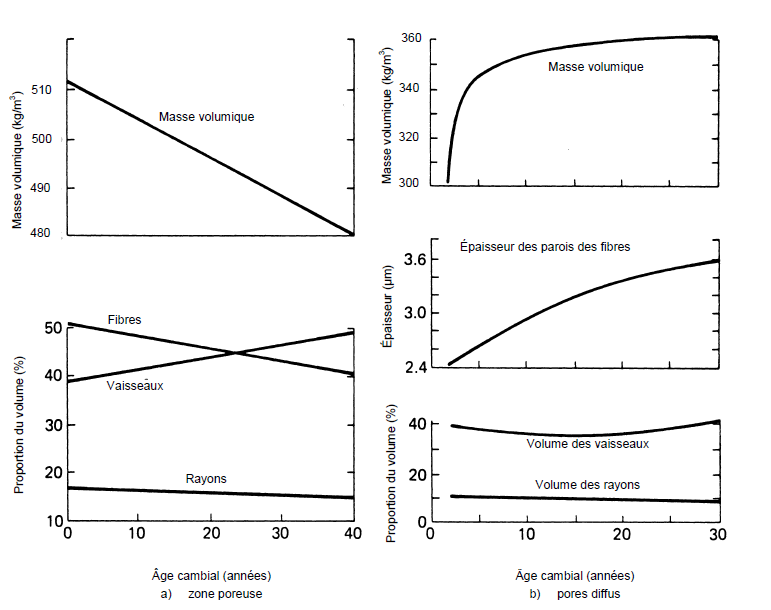
\includegraphics[scale=0.55]{img/ch7_densite_moelle_feuillus}
	\caption{Variation de la moelle vers l'écorce à 1,5 m de hauteur de la masse volumique, de la proportion des cellules et de l'épaisseur des parois cellulaires pour un feuillu à zone poreuse (\textit{Celtis laevigata}) et un feuillu à pores diffus (\textit{Salix nigra}) \cite{panshin1980textbook})}
	\label{fig:densite_moelle_feuillus}
\end{figure}


\subsubsection{Variabilité de la masse volumique selon la hauteur dans les tiges}

Il s'agit de l'axe de variation le moins bien décrit. Chez les résineux, pour un même âge cambial, $M_v$ tend parfois à diminuer de la base de la tige vers le haut (Figure~\ref{fig:densite_haut_dave}). Chez les feuillus, il est difficile de décrire des tendances générales. Retenez que l'âge cambial \hyperref[croissance_cernes]{(qui varie en fonction de la hauteur dans l'arbre)}, est le facteur le plus important de variation des propriétés du bois en fonction de la hauteur dans la tige.\\

\begin{figure}[h]
	\centering
	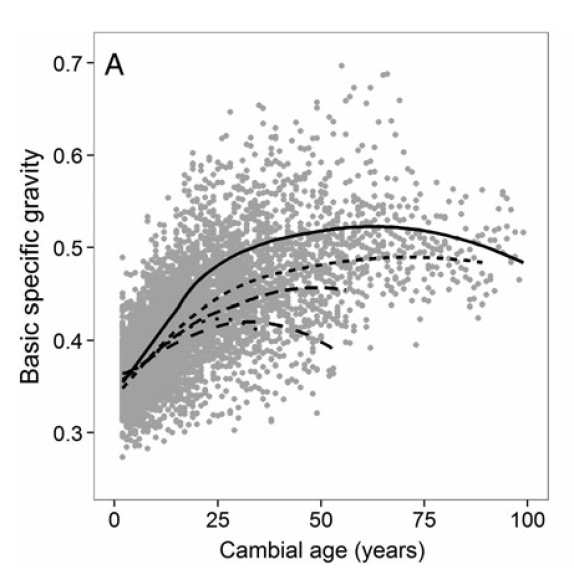
\includegraphics[scale=0.5]{img/ch7_densite_haut_dave}
	\caption{Variation de la masse volumique des cernes de pin sylvestre (\textit{Pinus sylverstris}) en fonction de l'âge cambial et de la hauteur dans l'arbre \cite{auty2014models}). La ligne pleine représente la base de la tige (1.3 m) et les traits pointillés représentent des niveau qui s'élèvent successivement dans l'arbre.}
	\label{fig:densite_haut_dave}
\end{figure}


\section{Variabilité des propriétés physiques et mécaniques du bois}

Les principales propriétés physiques et mécaniques des principaux bois commerciaux du Québec sont présentées au Tableau~\ref{tab:grostab}. 

\subsection{Masse volumique basale}

Résineux : de 335 à 549 kg/m\up{3}, CV de l'ordre de 10\%

Feuillus : de 374 à 597 kg/m\up{3}, CV de l'ordre de 6\%

\subsection{Module d'élasticité en flexion}

Résineux : de 9650 à 14300 MPa, CV de l'ordre de 20\%

Feuillus : de 11200 à 14100 MPa, CV de l'ordre de 17\%

\subsection{Module d'élasticité en compression parallèle au fil}

Résineux : de 9720 à 12300 MPa, CV de l'ordre de 23\%

Feuillus : de 12700 à 15400 MPa, CV de l'ordre de 18\%

\begin{table}[ht]
\centering
	\begin{tabular}{l c c c c c c c}
	\hline
Espèce	&	Mv basale	&	$\beta$R	&	$\beta$T	&	$\beta$T/$\beta$R	&	MOE flex.//	&	MOE comp.//	&	Dureté\\
&	(kg/m\up{3})	&	(\%)	&	(\%)	&		&	(à 12 \% H)	&	(à 12\% H)	&	(à 12\% H)\\
&		&		&		&		&	(MPa)	&	(MPa)	&	(N)\\
\hline
\hline
Épinette blanche	&	354	&	3,2	&	6,9	&	2,2	&	9930	&	11400	&	1880\\
&	(10,2)	&		&		&		&	(18,6)	&	(23,7)	&	(16,5)\\
Épinette noire	&	406	&	3,8	&	7,5	&	2,0	&	10400	&	12300	&	2430\\
&	(9,4)	&		&		&		&	(22,3)	&	(23,0)	&	(16,4)\\
Pin gris	&	421	&	4,0	&	5,9	&	1,5	&	10200	&	10500	&	2560\\
&	(8,8)	&		&		&		&	(19,8)	&	(23,9)	&	(15,7)\\
Pin blanc	&	364	&	2,5	&	6,3	&	2,5	&	9380	&	9720	&	1650\\
&	(11,3)	&		&		&		&	(19,9)	&	(22,5)	&	(21,1)\\
Sapin baumier	&	335	&	2,7	&	7,5	&	2,8	&	9650	&	9720	&	1820\\
&	(8,0)	&		&		&		&	(14,3)	&	(19,8)	&	(16,6)\\
Mélèze laricin	&	549	&	2,8	&	6,2	&	2,2	&	14300	&	10500	&	4210\\
&	(11,9)	&		&		&		&	(14,1)	&	(27,6)	&	(21,3)\\
\hline
Érable à sucre	&	597	&	4,6	&	8,8	&	1,9	&	14100	&	15400	&	7290\\
&	(5,2)	&		&		&		&	(13,9)	&	(14,7)	&	(12,3)\\
Bouleau jaune	&	559	&	5,8	&	7,1	&	1,2	&	14100	&	15200	&	5930\\
&	(5,4)	&		&		&		&	(22,3)	&	(23,0)	&	(16,6)\\
Chêne rouge	&	581	&	3,6	&	6,7	&	1,9	&	11900	&	13700	&	6170\\
&	(5,1)	&		&		&		&	(14,0)	&	(14,3)	&	(13,2)\\
Frêne d’Amérique	&	570	&	4,2	&	7,0	&	1,7	&	12800	&	13500	&	7050\\
&	(8,4)	&		&		&		&	(19,9)	&	(21,8)	&	(21,5)\\
P. faux-tremble	&	374	&	3,6	&	6,6	&	1,8	&	11200	&	12700	&	2140\\
&	(6,4)	&		&		&		&	(17,1)	&	(17,8)	&	(14,2)\\
	\hline
	\end{tabular}
\caption{Propriétés physiques et mécaniques des principales espèces commerciales du Québec. Les nombres entre parenthèses désignent le coefficient de variation (\%) (Écart-type divisé par la moyenne $\times$ 100)}
\label{tab:grostab}
\end{table}

\subsection{Dureté}

Résineux : de 1650 à 4210 N, CV de l'ordre de 18\%

Feuillus : de 2140 à 7290 N, CV de l'ordre de 16\%

\subsection{Stabilité dimensionnelle}

La stabilité dimensionnelle d'un bois peut être estimée à partir du rapport $\beta_T$/$\beta_R$. Plus ce rapport se rapproche de l'unité, moins le bois a tendance à se déformer avec les changements de teneur en humidité. Donc, si on doit choisir un bois pour une application nécessitant une grande stabilité, on doit vérifier deux choses :

\begin{enumerate}
\item les coefficients de retrait radial et tangentiel doivent être minimum.
\item le rapport $\beta_T$/$\beta_R$ doit aussi être minimum.
\end{enumerate}

$\beta_T$ est environ égal à $2\beta_R$. Il y a au moins deux théories pour expliquer cet état de chose. (1) L'effet des parois cellulaires du bois final : il y a plus de matière en direction tangentielle dans le bois final donc il y a plus de retrait en direction tangentielle. (2) Effet des rayons : les rayons constituent des structures ayant pour effet de limiter le retrait radial.

% ATTENTION : BIEN RELIRE CA parce que plein de symboles ont disparus
% Ok, c'est bon je crois

\section{Bilan}

Le tableau \ref{tab:bilan} résume l'ensemble des élément vus dans ce chapitre.

\begin{table}[p]

	\scriptsize
	
	\begin{tabular}{|b{0.4cm}|b{0.4cm}| m{4cm} m{4cm} m{4cm}|}
	
	\hline  &  & \bf Variation à l’intérieur des cernes annuels & \bf Variation entre les cernes annuels (section transversale) &  \bf Variation selon la hauteur \\ 
	\hline  \flip{\hspace{-0.7cm} \large Résineux} & \flip{\hspace{-0.65cm}\normalsize Trachéides} & 
	
	\begin{description}[leftmargin=0.2cm]
	\item[longueur] min. b.i.;  max. b.f.; 15\%
	\item[diamètre radial]  max. b.i.; min. b.f. 
	\item[angle microfibrilles] max. b.i.;  min. b.f.
	\item[teneur en cellulose]  min. b.i.;  max. b.f.
	\item[teneur en lignine] varie très peu
	\item[teneur en extractibles] diminue radialement
	\item[épaisseur des parois] min. b.i.;  max. b.f.
	\end{description}
	
	& 
	
	\begin{description}[leftmargin=0.2cm]
	\item[longueur] augmente dans les premières années de croissance; toujours plus court dans le b.i. que dans le b.f.
	\item[diamètre radial] augmente de la moelle vers l'écorce
	\item[diamètre tangentiel] augmente de la moelle vers l'écorce
	\item[épaisseur des parois] b.i.: augmente de la moelle vers l'écorce (20\%); b.f.: augmente de la moelle vers l'écorce ($\Delta$e  40\%).
	\item[angle microfibrilles] diminue de la moelle vers l'écorce
	\item[teneur en cellulose] augmente de la moelle vers l'écorce d'environ 45 à 65\% de $M_0$.
	\item[teneur en lignine] varie très peu
	\item[teneur en hémicelluloses] diminue de la moelle vers l'écorce
	\item[teneur en extractibles] diminue de la moelle vers l'écorce
	\end{description} 
	
	& 
	
	\begin{description}[leftmargin=0.2cm]
	\item[longueur] augmente de la souche vers la base de la cime et diminue par la suite jusqu'au sommet de l'arbre.
	\item[diamètre] augmente de la souche vers la base de la cime et diminue par la suite jusqu'au sommet de l'arbre.
	\item[épaisseur des parois] augmente de la souche vers la base de la cime et diminue par la suite jusqu'au sommet de l'arbre.
	\end{description} \\ 
	
	\hline \multirow{2}*{\flip{\large Feuillus \qquad}}  & \flip{\hspace{-0.7cm} \normalsize Vaisseaux} & 
	
	\begin{description}[leftmargin=0.2cm]
	\item[longueur] min. b.i.; max. b.f.;  l  10\% ou moins
	\item[diamètre] max. b.i.; min. b.f. chez les bois à zone poreuse et à pores semi-diffus
	\end{description}
	
	& 
	
	\begin{description}[leftmargin=0.2cm]
	\item[longueur] augmente de la moelle vers l'écorce
	\item[diamètre] augmente de la moelle vers l'écorce
	\item[angle microfibrilles] diminue de la moelle vers l'écorce
	\end{description}
	
	&  \\ 

	
	\cline{2-5} & \flip{\hspace{-0.5cm}  \normalsize Fibres} & 
	
	\begin{description}[leftmargin=0.2cm]
	\item[longueur] min. b.i.;  max. b.f.; l  30 à 100\%
	\item[angle microfibrilles] max. b.i.; min. b.f.
	\end{description} 
	
	& 
	
	\begin{description}[leftmargin=0.2cm]
	\item[longueur] augmente radialement
	\item[épaisseur des parois] augmente de la moelle vers l'écorce
	\item[angle microfibrilles] diminue de la moelle vers l'écorce
	\end{description}
	
	&  
	
	\begin{description}[leftmargin=0.2cm]
	\item[longueur] augmente de la souche vers la base de la cime et diminue par la suite jusqu'au sommet de l'arbre.
	\item[diamètre] diminue de la souche jusqu'au sommet de l'arbre
	\item[épaisseur des parois] diminue de la souche jusqu'au sommet de l'arbre
	\end{description}\\ 
	\hline 
	\end{tabular} 
	
	\caption{Tableau résumé de notions vues dans ce chapitre}
	\label{tab:bilan}
\end{table}


%Références
%
%
%
%Panshin, A.J.; de Zeeuw, C. 1980. Textbook of wood technology. Fourth edition. McGraw-Hill Book Co. New York. 722 p. 
%
%
%
%Jessome, A.P. 1977. Strength and related properties of woods grown in Canada. Forintek Canada Corp. 37 p.
